\section{下板验证}

\subsection{编译与烧录流程}

\begin{enumerate}[leftmargin=2em]
    \item \textbf{软件编译}：在 WSL 中执行 \texttt{bash software/build.sh}，依次编译 BootLoader 与 \texttt{$\mu$C/OS-II + 用户程序}，链接生成 \texttt{ucosii.bin}，再由 \texttt{BinMerge.exe} 合成最终 \texttt{OS.bin}。
    \item \textbf{硬件综合}：Vivado 2024.2 打开 \texttt{exp3.xpr}，重新生成 IP（MIG、clk\_wiz），依次 Run Synthesis $\to$ Run Implementation $\to$ Generate Bitstream，得到 \texttt{openmips\_min\_sopc.bit}。
    \item \textbf{烧录}：Hardware Manager 连接开发板，Add Configuration Memory Device 选 \textbf{\texttt{s25fl128sxxxxx0-spi-x1\_x2\_x4}}（板载 Spansion Flash），把 \texttt{OS.bin} 写入（Erase + Program + Verify）；再 Program Device 下载比特流启动 FPGA。
    \item \textbf{运行}：PC 运行 \texttt{python play.py}，自动检测 \texttt{COM3} 启动 pygame。
\end{enumerate}

\subsection{验证结果}

\textbf{(1) 串口帧验证}：先用 \texttt{debug\_rx.py} 验证 FPGA 发帧与协议。按下中键前处于 READY 态，终端持续打印蛇身 ASCII 位图，蛇头（\texttt{@@}）、蛇身（\texttt{[]}）、食物（\texttt{**}）位置正确，如图~\ref{fig:debug}。

\begin{figure}[H]
    \centering
    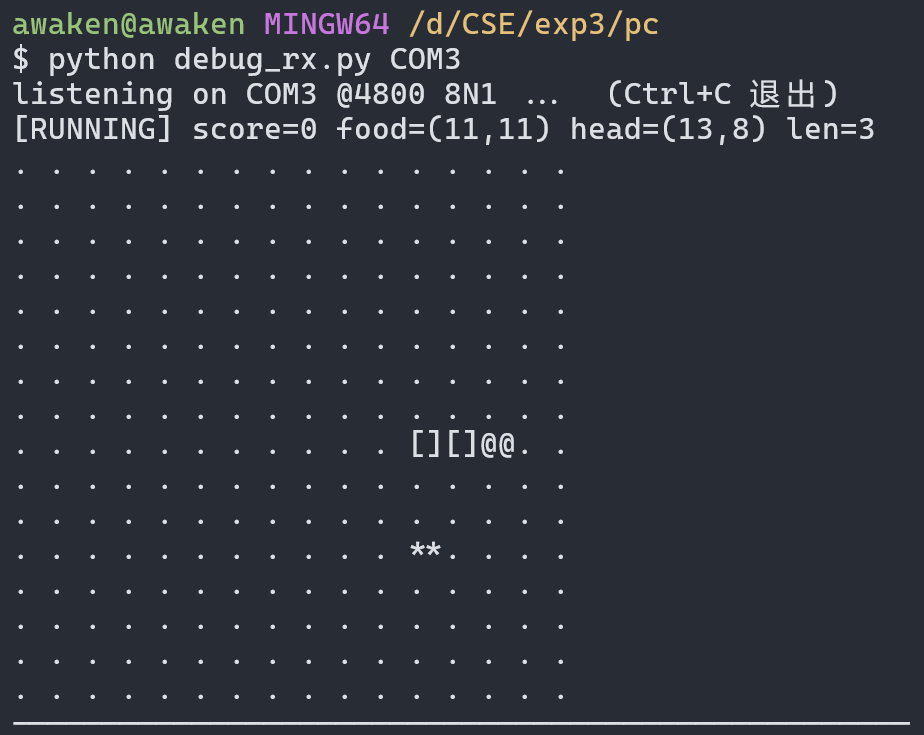
\includegraphics[width=0.75\textwidth]{img/debug.png}
    \caption{串口帧调试输出（debug\_rx.py）}
    \label{fig:debug}
\end{figure}

\textbf{(2) pygame 游戏画面}：进入 GUI 后按中键开始，蛇以约 5 格/秒的速度移动，方向按钮实时转向，吃到食物变长、分数 +1。如图~\ref{fig:gui} 为运行中画面。

\begin{figure}[H]
    \centering
    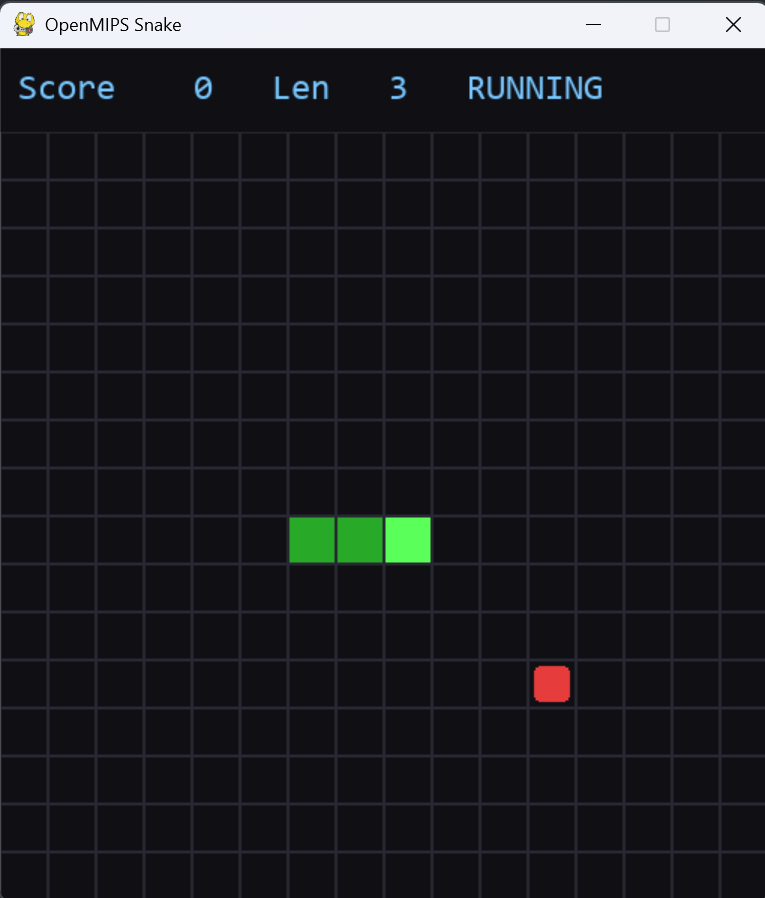
\includegraphics[width=0.7\textwidth]{img/gui.png}
    \caption{pygame 运行中画面}
    \label{fig:gui}
\end{figure}

\textbf{(3) 边界回环}：蛇触及任一边界不再 Game Over，而是从对侧穿出（验证回环边界逻辑）。

\begin{figure}[H]
    \centering
    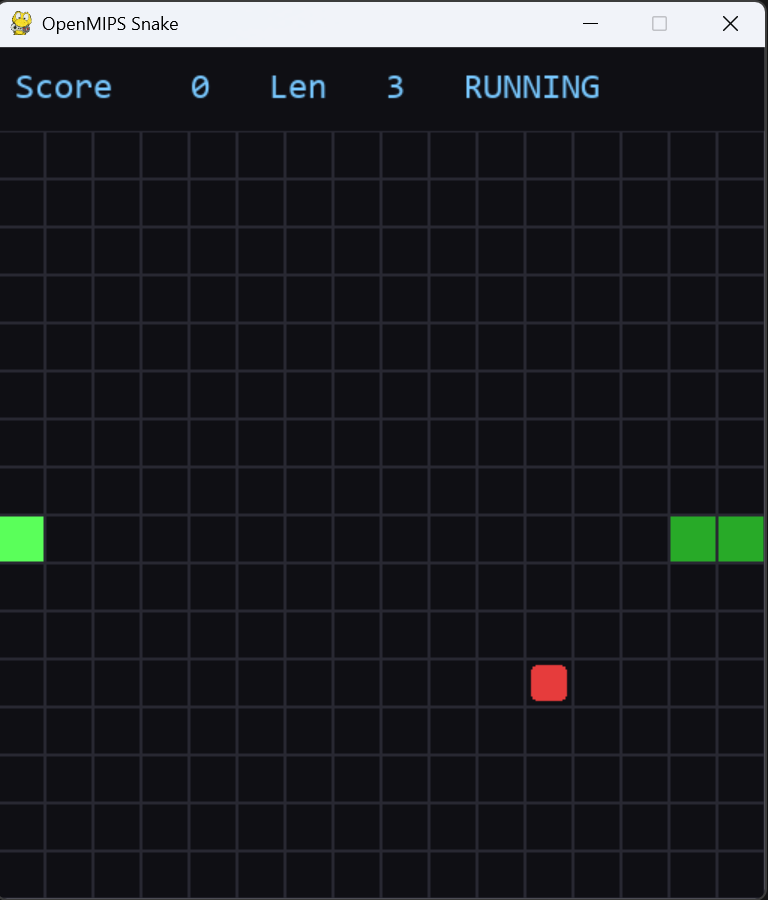
\includegraphics[width=0.7\textwidth]{img/loop.png}
    \caption{边界回环：蛇头从一侧穿出，从对侧穿进}
    \label{fig:loop}
\end{figure}

\textbf{(4) Game Over 与重开}：蛇头撞到自身时进入 GAME OVER 态，画面停止；按中键（BTNC）重开新局。

\begin{figure}[H]
    \centering
    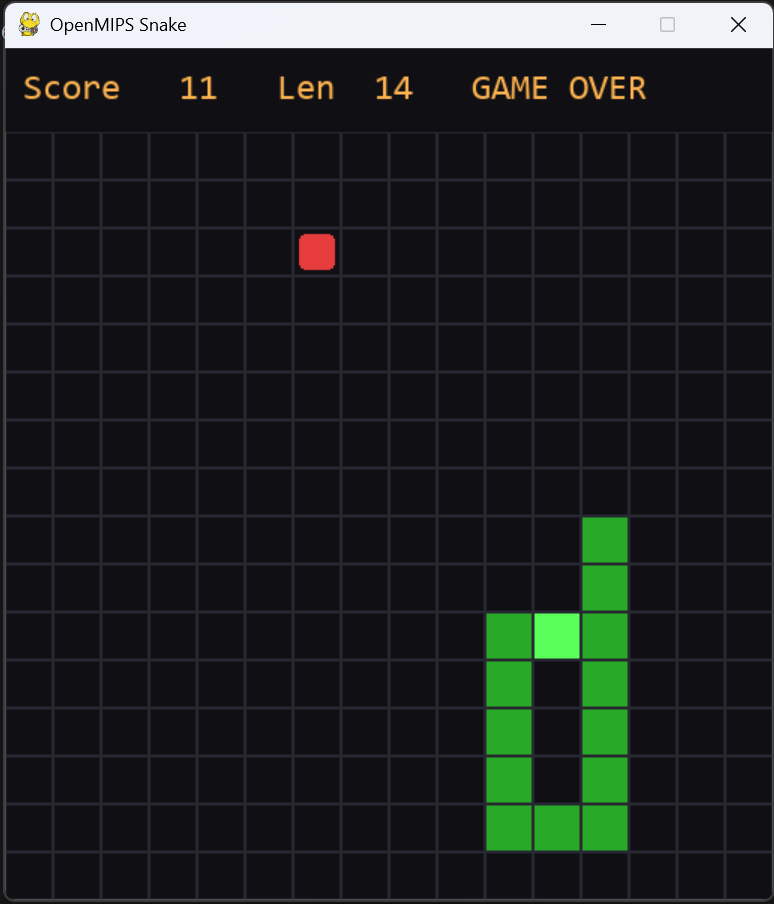
\includegraphics[width=0.7\textwidth]{img/over.png}
    \caption{Game Over 画面}
    \label{fig:over}
\end{figure}

\textbf{(5) 数码管分数}：板上七段数码管同步显示分数（十六进制），随吃食递增，如图~\ref{fig:seg}。

\begin{figure}[H]
    \centering
    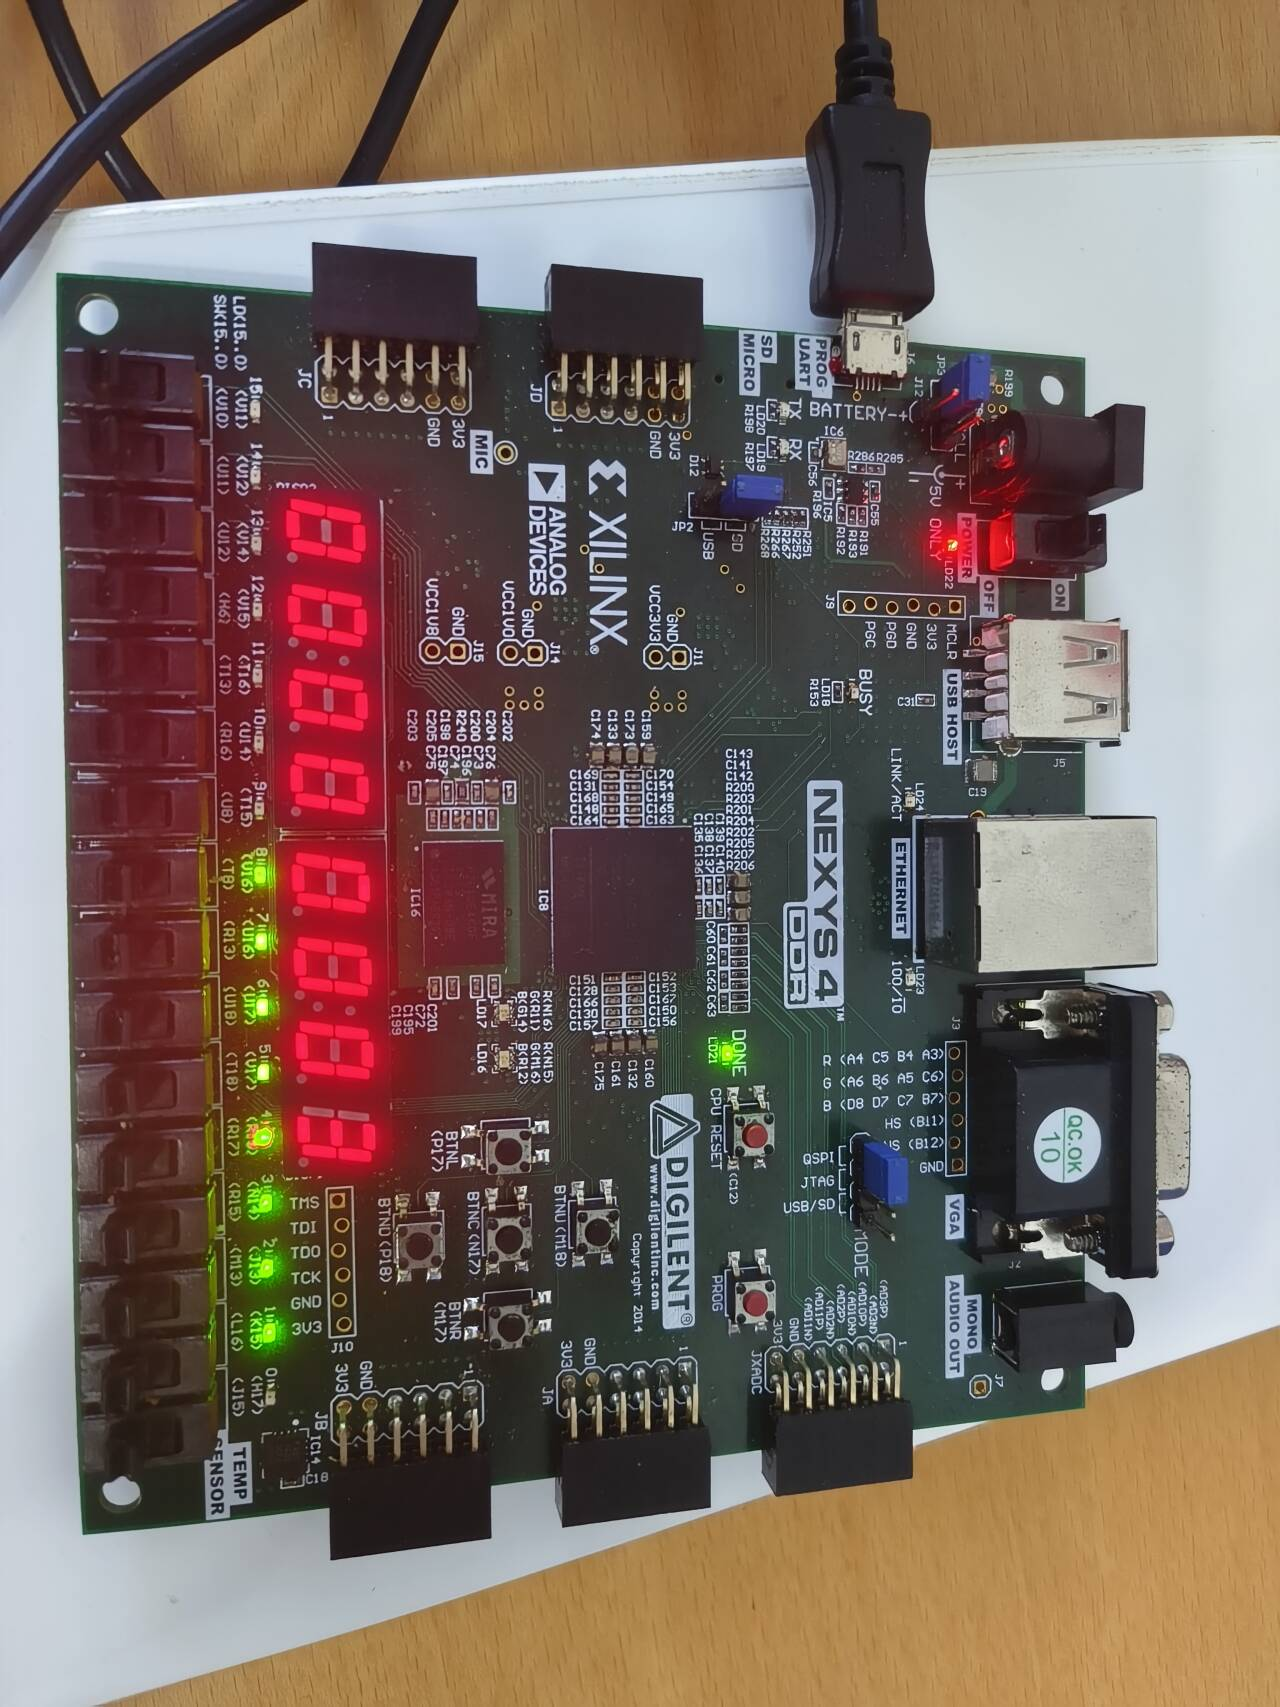
\includegraphics[width=0.5\textwidth]{img/seg.jpg}
    \caption{数码管显示分数（开发板实物）}
    \label{fig:seg}
\end{figure}

\subsection{验证结论}

板载按钮（中/上/下/左/右）全部生效，UART 通信稳定，画面渲染流畅，数码管同步显示分数，边界回环与速度减半均符合预期。\textbf{全部功能验证通过}。
